\documentclass[11pt]{beamer}
\usepackage[utf8]{inputenc}
\usepackage[T1]{fontenc}
\usepackage{lmodern}
\usetheme{Madrid}
\usepackage{tabularx}
\usepackage{booktabs}
\bibliographystyle{apalike}
%\usepackage[style=apa, backend=biber, natbib=true]{biblatex}
%\addbibresource{references.bib}
%\bibliography{document}
\begin{document}
	\author[Group Nine]{KALONG BONIFACE \\
		   FUGAH SELETEY MITCHELL\\
		  			  SUPERVISER: MR JUSTIES AMAYOR KESSIE	}  
\title[Proposal]{THE VARIABILITY CLIMATE CHANGE IS RESPONSIBLE FOR IN VEGETATION LOSS IN GHANA}
	\subtitle{Quantifying The Status of Galamsey With Time Series Analysis}
	\logo{\includegraphics[scale=0.05]{images/logo2}}
	\institute[UENR]{Department of Mathematics and Statistics\\University Of Energy and Natural Resource,Sunyani}
	\date{\today}
	%\subject{Proposal}
	%\setbeamercovered{transparent}
	%\setbeamertemplate{navigation symbols}{}
	\begin{frame}
		\maketitle
	\end{frame}
	\begin{frame}
		\frametitle{Outline Of Presentation}
		\begin{itemize}
			\item Introduction
			\item Problem Statement
			\item Objective
			\item Methodology
			\item Reference
		\end{itemize}
	\end{frame}

	\begin{frame}
		\frametitle{INTRODUCTION}
		\begin{block}{}
One would anticipate that the majority of emerging nations, which are still in the early stages of economic development and growth, would have a high forest cover and little deforestation. This, however, has not been the case. Ghana is a lower-middle-income nation that is still working toward middle-income classification. However, it has already begun to see a deforestation rate that is comparable to that of middle-income countries. The rapid population expansion, clearing of field for Galamsey operation,increased domestic need of wood for things like fuel, furniture, construction, and timber exports have all contributed to this trend, Bush fires in the 1980s, climate change, and lax law enforcement have all had an impact. \\
       \end{block}
	\end{frame}
     \begin{frame}
     	\frametitle{Introduction Con't}
     	\begin{block}{}
     		The purpose of this paper is to establish an understanding in time series analysis on remotely sensed data. Which will introduced us to the fundamentals of time series modeling, including decomposition, autocorrelation and modeling historical changes in Galamsey Operation in Ghana, the Cause,Dangers and it's Environmental impact 
     	\end{block}
     
     \end{frame}
 \begin{frame}
 	\frametitle{Introduction Con't}
 	\begin{block}{}
 	Galamsey also known as "gather them and sell",\emph{Owusu-Nimo2018} is the term given by local Ghanaian for illegal small-scale gold mining in Ghana . The major cause of Galamsey is unemployment among the youth in Ghana \emph{Gracia2018}. Young university graduates rarely find work and when they do it hardly sustains them. The result is that these youth go the extra mile to earn a living for themselves and their family.
 	
 	\end{block}
 	
 \end{frame}
\begin{frame}
	
	\begin{block}{PROBLEM STATEMENT}
		
		The Footprint of Galamsey is Spreading at a very faster rate, causing vegetation loss.Other factors accounting to vegetation loss may largely include climate change,urban and exurban development, bush fires. But not much works or research has been done to tell the extent to which Galamsey causes vegetation loss. This research attempts to segregate the variability climate is responsible for in vegetation loss so as to attribute the residual variability to Galamsey and other related activities such as bush-fires etc.
	
	\end{block}
\end{frame}
\begin{frame}
	\begin{block}{Research Questions}
To address the challenge of the vegetation variability in this work, the following several statements were formed:

\begin{itemize}
	\item  Are there any changes in vegetation cause by Galamsey and Climate change in Ghana?
	
	\item Is there any relationship between vegetation and land surface temperature in Ghana?
\end{itemize}
	\end{block}
\end{frame}
\begin{frame}
	\begin{block}{OBJECTIVE}
	
	The purpose is to establish an understanding in time series analysis on remotely sensed data. We will be introduced to the fundamentals of time series modeling, including decomposition, auto-correlation and modeling historical changes.
	
	\begin{itemize}
		\item Perform time series analysis on satellite derived vegetation indices
		
		\item Estimate the extent to which Galamsey causes vegetation loss in Ghana.
		
		\item Dissociate or single out the variability climate is responsible for in vegetation loss
	\end{itemize}
	\end{block}
\end{frame}
\begin{frame}
	\begin{block}{Significance Of The Study}
		In this study, we want to examine the effects of climatic change on Ghana's vegetation during these thirty years.
		
		\begin{itemize}
		\item 	This study allows us to explore climatic differences and climate-related drivers.
		\item	It offers a chance to research how climatic variability affects the ecosystem and human health. 
		\item	This study explores historical and projected vegetation and climate data, by sector, impacts, key vulnerabilities and what adaptation measures can be taken.
		\item	It also explores the overview for a general context of how climate change is affecting Ghana.
		\end{itemize}
	\end{block}
\end{frame}
\begin{frame}
	\begin{block}{Limitation Of The Study}		
	
The goal of time series modeling is to employ the simplest model feasible to account for as much data as possible while still developing an explanatory model of the data that does not over-fit the issue set.

\begin{itemize}
	\item Missing Data
	\item It is almost certain that data from distant sensing will not provide the same level of precision.
	\item Atmospheric factors can distort the visual findings, causing the vegetation's color to shift dramatically from image to image as a result of atmospheric factors (fog, ground moisture, cloud cover)
\end{itemize}
	\end{block}
\end{frame}
\begin{frame}
	\frametitle{Data}
		
The Satellite (MOD13) provide consistent,and spatial time series comparisons of global vegetation conditions that can be used to monitor the Earth’s  photosynthetic vegetation activity in support of  \textbf{change detection}, and biophysical interpretations.For this analysis, we will be using the MOD13Q1 V6 product which contains the Enhanced Vegetation Index (EVI).
	% TODO: \usepackage{graphicx} required
	\begin{figure}
		\centering
		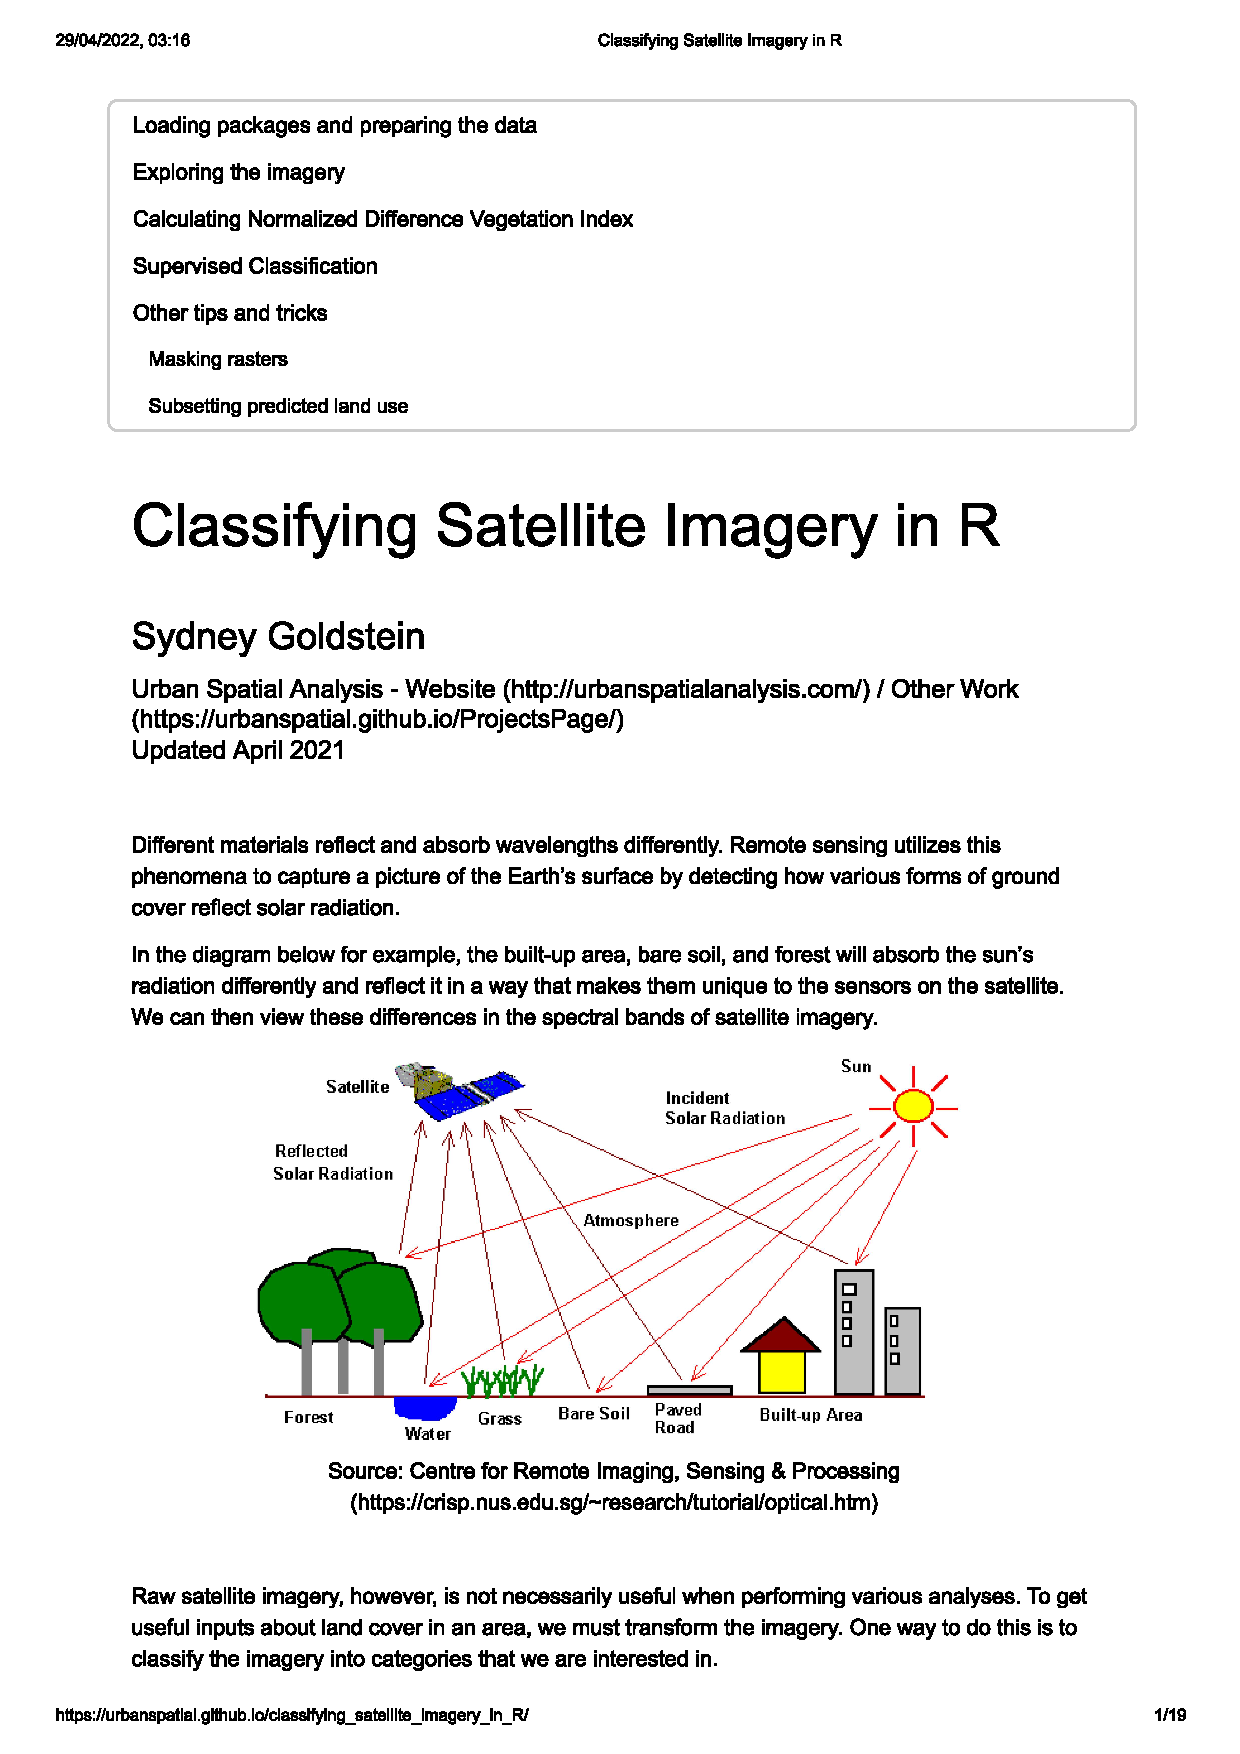
\includegraphics[width=0.7\linewidth]{images/classification}
		\caption{}
		\label{fig:classification}
	\end{figure}
	
\end{frame}

\begin{frame}
	\frametitle{Data}
% TODO: \usepackage{graphicx} required
\begin{figure}
	\centering
	\includegraphics[width=0.7\linewidth]{images/EVI}
	\caption{}
	\label{fig:evi}
\end{figure}

	
NIR, Red, and Blue are the surface reflectances that have been fully or partially adjusted for Rayleigh scattering and ozone absorption due to the atmosphere; C1 and C2 are the coefficients of the aerosol resistance term (which uses the blue band to correct for aerosol influences in the red band); L is the canopy background adjustment for correcting the nonlinear, differential NIR and red radiant transfer through a canopy; and G is a gain or scaling factor. The MODIS EVI algorithm's chosen coefficients are L=1, C1=6, C2=7.5, and G=2.5.
	
\end{frame}

\begin{frame}
	\frametitle{Data}
	% TODO: \usepackage{graphicx} required
	\begin{figure}
		\centering
		\includegraphics[width=0.7\linewidth]{images/DataExtraction}
		\caption{Data Extraction from Google Earth Engine}
		\label{fig:dataextraction}
	\end{figure}
	
	Instead of analyzing the imagery directly, we will summarize the mean EVI values. We will apply a smoothing strategy using an ARIMA function to fix the situation where some cells may not have EVI for a particular month. Once NA values have been eliminated, the time series will be divided to eliminate seasonality before the normalized data is fitted using a linear model. We will go to classify our data on the map and map it after we have extracted the linear trend.
	
\end{frame}


\begin{frame}
	\frametitle{Methodology}
we will first collect data from Google Earth Engine in order to choose  EVI values and Climate Change data.
% TODO: \usepackage{graphicx} required
\begin{figure}
	\centering
	\includegraphics[width=0.7\linewidth]{images/Rplot}
	\caption{Creating Hex cell(Polygons) on the Study Area}
	\label{fig:rplot}
\end{figure}
\end{frame}

\begin{frame}
	\begin{block}{Methodology Cont'}
		% TODO: \usepackage{graphicx} required
		\begin{figure}
			\centering
			\includegraphics[width=0.7\linewidth]{images/Methodology}
			\caption{Flow Chart to Galamsey Detection}
			\label{fig:methodology}
		\end{figure}
		
	\end{block}
\end{frame}
\begin{frame}
	\begin{block}{Methodology Cont'}
		\begin{itemize}
		\item[*] To help machine learning classifiers works better with time series data .
		\item[*] Local features or patterns in time series can be found and combined to address challenges involving time-series categorization.
		\item[*] Then, a method to discover patterns that are helpful for classification is suggested.
		\item[*] combine these patterns to create computable categorization rules. 
	\end{itemize}
\textbf{vector autoregression (VAR) }\\

It is of the form 
$y_{t} = A_{1}y_{t-1} + A_{2}y_{t-2} +\cdot+A_{p}y_{t-p}+ CD_{t} + \mu $\\
where;\\
\begin{itemize}
	\item  $ y_{t} = \left( y_{1t},y_{2t},...,y_{kt}\right)'$ is a vector of K observable endogenous variables \\
\item    For the purposes of this study, yt = $(EVI_{t}, Temperature_{t}, Rain_{}, Precipitation_{t},Drought_{t},Evaporation_{t})'$
\end{itemize}
 where EVI denotes the value of vegetation conditions  each month
	\end{block}
\end{frame}
\begin{frame}
	\frametitle{explanation}
	\begin{columns}
		\begin{column}{0.5\textwidth}
			\begin{itemize}
				\item Augmented Dickey Fuller unit root test
				\item Lag Selection using information Criteria (AIC,HQ,SC,FPE)
				\item Causality Test (Granger Causality)
				\item Impose Analysis
				\item Decomposition of Variance (FEVD)
			\end{itemize}
		\end{column}
		\begin{column}{0.5\textwidth}  %%<--- here
					% TODO: \usepackage{graphicx} required
					\begin{center}
						\includegraphics[width=0.7\linewidth]{images/Accuracy}
					\end{center}
		\end{column}
	\end{columns}
\end{frame}
\begin{frame}{Result}
% TODO: \usepackage{graphicx} required
\begin{figure}
	\centering
	\includegraphics[width=0.7\linewidth]{images/TimeSeries}
	\caption{}
	\label{fig:timeseries}
\end{figure}
\end{frame}
\begin{frame}{Result Causality}
	\begin{table}[]
		\label{Optimal lag}
		\caption{Granger causality tests.}
		\centering
		\small
		\addtolength{\tabcolsep}{-4pt}
		\begin{tabularx}{\textwidth}{@{}lllll@{}}
			\hline
			Cause variable &Null hypothesis& F-value& p-value& Decision\\
			\hline\hline
			Precipitation	& does not Granger-cause EVI &2.1563  & 0.01464  & Reject the null hypothesis  \\
			\hline
			Evaporation	& does not Granger-cause EVI & 1.5398 & 0.1112 &Fail to Reject the null hypothesis  \\
			\hline
			TempMin	&  does not Granger-cause EVI&3.0049  & 0.0006276 &Reject the null hypothesis  \\
			\hline
			TempMax	& does not Granger-cause EVI&2.7462  & 0.001685 &Reject the null hypothesis  \\
			\hline
			Drought	& does not Granger-cause EVI & 0.9235 & 0.5241 &Fail to Reject the null hypothesis \\
			\hline
		\end{tabularx}
	\end{table}
\end{frame}
\begin{frame}{Result}
	% TODO: \usepackage{graphicx} required
	\begin{figure}
		\centering
		\includegraphics[width=0.7\linewidth]{images/impose}
		\caption{}
		\label{fig:impose}
	\end{figure}
	
\end{frame}

\begin{frame}{Result}
	\begin{figure}
		\centering
		\includegraphics[width=0.7\linewidth]{images/fevd}
		\caption{}
		\label{fig:fevd}
	\end{figure}
\end{frame}
\begin{frame}{Discussion}
	The Granger and immediate causality tests reveal that only three climate factors have an impact on malaria. The impulse response analyses show that the ninth, third, and tenth months, respectively, had the strongest favorable effects of maximum temperature, relative humidity, and rainfall on malaria. With less than 20\% of the variability in the trend of EVI being explained by historical innovations in Climate Change, the decomposition of predicted variance shows varied degrees of EVI dependence on climatic variables. Policymakers can utilize the study's findings to assist them develop policies by understanding how climatic variability affects the incidence of EVI in the Study Area.

\end{frame}
\begin{frame}
	\frametitle{References}
	\begin{thebibliography}{9}
		\bibitem{Hawkins1973}Šoltés, E., Zelinová, S., $\&$ Bilíková, M. (2019). General linear model: An effective tool for analysis of claim severity in motor third party liability insurance. STATISTICS, 13,
		\bibitem{citekey}Yau, K., Yip, K., $\&$ Yuen, H. K. (2003). Modelling repeated insurance claim frequency data using the generalized linear mixed model. Journal of Applied Statistics, 30(8), 857-865,	
		\bibitem{Jiang}Jiang, J., $\&$ Nguyen, T. (2007). Linear and generalized linear mixed models and their applications (Vol. 1). New York: Springer.
	\end{thebibliography}
\end{frame}


\end{document}